\documentclass{article}
\usepackage[utf8x]{inputenc}
\usepackage{ucs}
\usepackage{amsmath} 
\usepackage{amsfonts}
\usepackage{marvosym}
\usepackage{wasysym}
\usepackage{upgreek}
\usepackage[english,russian]{babel}
\usepackage{graphicx}
\usepackage{float}
\usepackage{textcomp}
\usepackage{hyperref}
\usepackage{geometry}
  \geometry{left=2cm}
  \geometry{right=1.5cm}
  \geometry{top=1cm}
  \geometry{bottom=2cm}
\usepackage{tikz}
\usepackage{ccaption}
\usepackage{multicol}

\hypersetup{
   colorlinks=true,
   citecolor=blue,
   linkcolor=black,
   urlcolor=blue
}

\usepackage{listings}
%\setlength{\columnsep}{1.5cm}
%\setlength{\columnseprule}{0.2pt}

\usepackage[absolute]{textpos}

\usepackage{colortbl,graphicx,tikz}
\definecolor{X}{rgb}{.5,.5,.5}


\begin{document}
\pagenumbering{gobble}
\lstset{
  language=C,                % choose the language of the code
  basicstyle=\linespread{1.1}\ttfamily,
  columns=fixed,
  fontadjust=true,
  basewidth=0.5em,
  keywordstyle=\color{blue}\bfseries,
  commentstyle=\color{gray},
  stringstyle=\ttfamily\color{orange!50!black},
  showstringspaces=false,
  numbersep=5pt,
  numberstyle=\tiny\color{black},
  numberfirstline=true,
  stepnumber=1,                   % the step between two line-numbers.        
  numbersep=10pt,                  % how far the line-numbers are from the code
  backgroundcolor=\color{white},  % choose the background color. You must add \usepackage{color}
  showstringspaces=false,         % underline spaces within strings
  captionpos=b,                   % sets the caption-position to bottom
  breaklines=true,                % sets automatic line breaking
  breakatwhitespace=true,         % sets if automatic breaks should only happen at whitespace
  xleftmargin=.2in,
  extendedchars=\true,
  keepspaces = true,
}
\lstset{literate=%
   *{0}{{{\color{red!20!violet}0}}}1
    {1}{{{\color{red!20!violet}1}}}1
    {2}{{{\color{red!20!violet}2}}}1
    {3}{{{\color{red!20!violet}3}}}1
    {4}{{{\color{red!20!violet}4}}}1
    {5}{{{\color{red!20!violet}5}}}1
    {6}{{{\color{red!20!violet}6}}}1
    {7}{{{\color{red!20!violet}7}}}1
    {8}{{{\color{red!20!violet}8}}}1
    {9}{{{\color{red!20!violet}9}}}1
}
\newpage

\title{Семинар \#8: Указатели и динамическое выделение памяти. Домашнее задание.\vspace{-5ex}}\date{}\maketitle
\section*{Память}
\textbf{Задача \#1:} Как выглядит память, инициализируемая при создании следующих переменных (в системе с порядком байт Little Endian):
\begin{multicols}{2}
\begin{enumerate}
\item \texttt{int a = 0x11223344;}
\item \texttt{int b = 123456789;}
\item \texttt{int array[3] = \{10, 2000, 65535}\};
\item \texttt{char str[8] = ''Hello``};
\item \texttt{float x = -15.91};
\item \texttt{double y = -15.91};
\item
\begin{verbatim}
struct data
{
    char str[5];
    int number;
};
struct data c = {"Cat", 100000};
\end{verbatim}
\end{enumerate}
\end{multicols}
Память представить в виде последовательности 2-значных шестнадцатиричных чисел. Например число \\
\texttt{int a = 757004;} будет храниться в памяти как \texttt{0x54, 0x82, 0x73, 0x00}. \\ \\
\textit{Подсказка:} Чтобы проверить, как будет выглядеть память, можно создать указатель типа \texttt{char*} на эту память и распечатать каждый байт в виде шестнадцатиричного числа:
\begin{lstlisting}
char* p = (char*)&a;
for (int i = 0; i < sizeof(a); ++i)
{
    printf("0x%02hhx ", p[i]);
}
\end{lstlisting}

\section*{Указатели}

\subsection*{Указатель на \texttt{int}}
\begin{multicols}{2}
\begin{lstlisting}
	int a = 1234;
	int* p = &a;
\end{lstlisting}
\columnbreak
\begin{center}
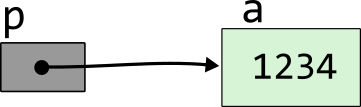
\includegraphics[scale=1]{../../images/pointer_schemes/pointer_to_int.png}
\end{center}
\end{multicols}
\textbf{Задача \#2:} Удвойте значение переменной \texttt{a}, используя только указатель \texttt{p}.

\subsection*{Указатель на указатель на \texttt{int}}

\begin{multicols}{2}
\begin{lstlisting}
	int a = 1234;
	int* p = &a;
	int** q = &p;
\end{lstlisting}
\columnbreak
\begin{center}
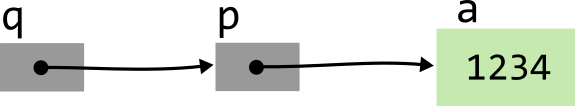
\includegraphics[scale=1]{../../images/pointer_schemes/pointer_to_pointer_to_int.png}
\end{center}
\end{multicols}
\textbf{Задача \#3:} Удвойте значение переменной \texttt{a}, используя только указатель \texttt{q}.

\newpage
\subsection*{Указатель на элемент массива}
\begin{multicols}{2}
\begin{lstlisting}
int main()
{
  int array[6] = {4, 8, 15, 16, 23, 42};
  int* p = &array[2];
}
\end{lstlisting}
\columnbreak
\begin{center}
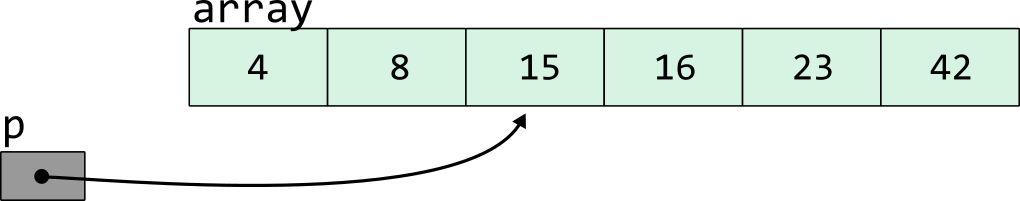
\includegraphics[scale=0.75]{../../images/pointer_schemes/pointer_to_array_of_ints.png}
\end{center}
\end{multicols}

\textbf{Задача \#4:} Удвойте значение \texttt{array[1]}, используя только указатель \texttt{p}.

\subsection*{Указатель на структуру}
\begin{multicols}{2}
\begin{lstlisting}
#include <stdio.h>
struct date
{
	int day;
	int month;
	int year;
};
\end{lstlisting}
\columnbreak
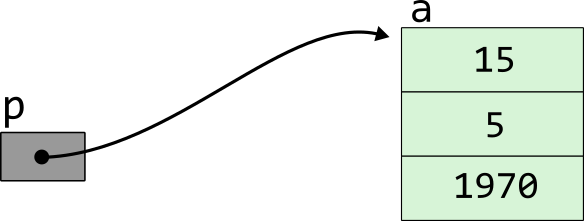
\includegraphics[scale=1]{../../images/pointer_schemes/pointer_to_struct_date.png}
\end{multicols}
\vspace{-5ex}
\begin{lstlisting}
int main()
{
	struct date a = {15, 5, 1970};
	struct date* p = &a;
	printf("%d %d %d\n", a.day, (*p).day, p->day);
}
\end{lstlisting}
\textbf{Задача \#5:} Удвойте значение поля \texttt{year}, используя только указатель \texttt{p}.

\subsection*{Указатель на структуру немного сложнее}
\begin{multicols}{2}
\begin{lstlisting}
#include <stdio.h>
struct movie
{
	char title[50];
	float rating;
	struct date release_date;
};
typedef struct movie Movie;
\end{lstlisting}
\columnbreak
\begin{center}
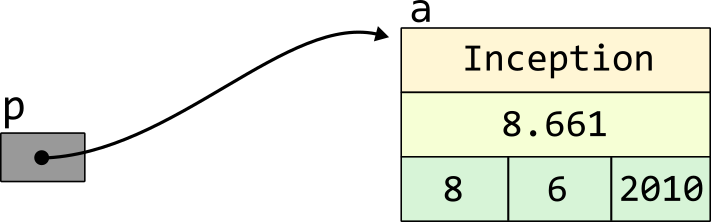
\includegraphics[scale=1]{../../images/pointer_schemes/pointer_to_struct_movie.png}
\end{center}
\end{multicols}
\begin{lstlisting}
int main()
{
	Movie a = {"Inception", 8.661, {8, 6, 2010}};
	Movie* p = &a;
}
\end{lstlisting}
\textbf{Задача \#6:} Удвойте значение поля \texttt{rating}, используя только указатель \texttt{p}.\\
\textbf{Задача \#7:} Удвойте значение поля месяца выхода фильма, используя только указатель \texttt{p}.

\subsection*{Указатель на массив структур}
\begin{lstlisting}
#include <stdio.h>
struct movie
{
	char title[50];
	float rating;
	struct date release_date;
};
typedef struct movie Movie;

int main()
{
	Movie a[3] = {{"Inception", 8.661, {8, 6, 2010}}, 
	              {"Green Mile", 9.062, {6, 12, 1999}}, 
	              {"Leon", 8.679, {14, 9, 1994}}};
	Movie* p = &a[1];
}
\end{lstlisting}

\vspace{-59ex}
\begin{center}
\quad\quad\quad\quad\quad\quad\quad\quad\quad\quad\quad\quad\quad\quad\quad\quad\quad\quad\quad\quad\quad\quad\quad
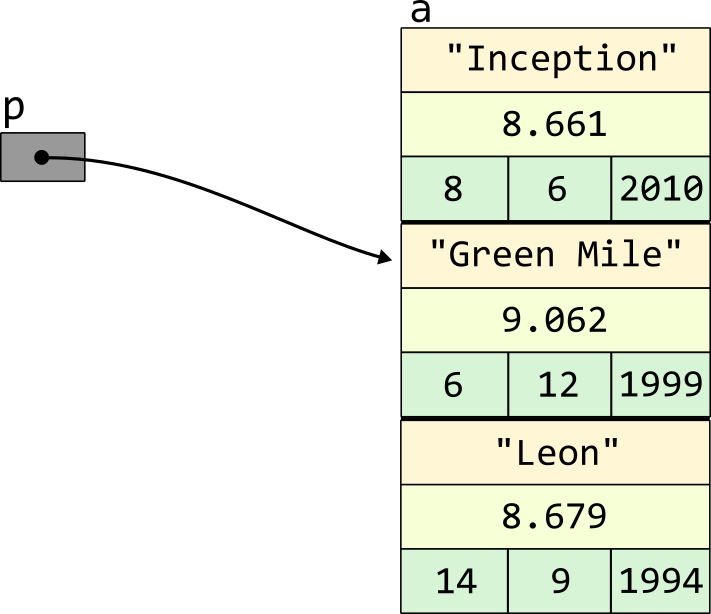
\includegraphics[scale=1]{../../images/pointer_schemes/pointer_to_array_of_struct_movie.png}
\end{center}
\textbf{Задача \#8:} Удвойте значение рейтинга фильма \texttt{Inception}, используя только указатель \texttt{p}.\\
\textbf{Задача \#9:} Удвойте значение года выхода фильма \texttt{Leon}, используя только указатель \texttt{p}.


\newpage
\section*{Memory allocation}
Основные функции для динамического выделения памяти:
\begin{itemize}
\item \texttt{void* malloc(\textbf{size\_t} n)} -- выделяет n байт и возвращает указатель \texttt{void*}
на начало этой памяти \\
\item \texttt{void free(\textbf{void*} p)} -- освобождает выделенную память\\
\item \texttt{void* realloc(\textbf{void*} p, \textbf{size\_t} new\_n)} -- перевыделяет выделенную память\\
\end{itemize}
\begin{lstlisting}
#include <stdio.h>
#include <stdlib.h>

int main()
{
	int number_of_elements = 20;
	int* p = (int*)malloc(number_of_elements * sizeof(int)); 

	free(p);
}
\end{lstlisting}

\subsection*{Указатель на массив структур, выделенный в куче}
\begin{lstlisting}
#include <stdio.h>
struct movie
{
	char title[50];
	float rating;
	struct date release_date;
};
typedef struct movie Movie;

void set_movie(Movie* pm, char* title, float rating, int day, int month, int year)
{
	pm->title = (char*)malloc(strlen(title) + 1);
	strcpy(pm->title, title);
	pm->rating = rating;
	pm->release_date.day = day;
	pm->release_date.month = month;
	pm->release_date.year = year;
}

int main()
{
	Movie* p = (Movie*)malloc(3 * sizeof(Movie));
	set_movie(p, "Inception", 8.661, 8, 6, 2010);
	set_movie(p + 1, "Green Mile", 9.062, 6, 12, 1999);
	set_movie(p + 2, "Leon", 8.679, 14, 9, 1994);
}
\end{lstlisting}
\begin{center}
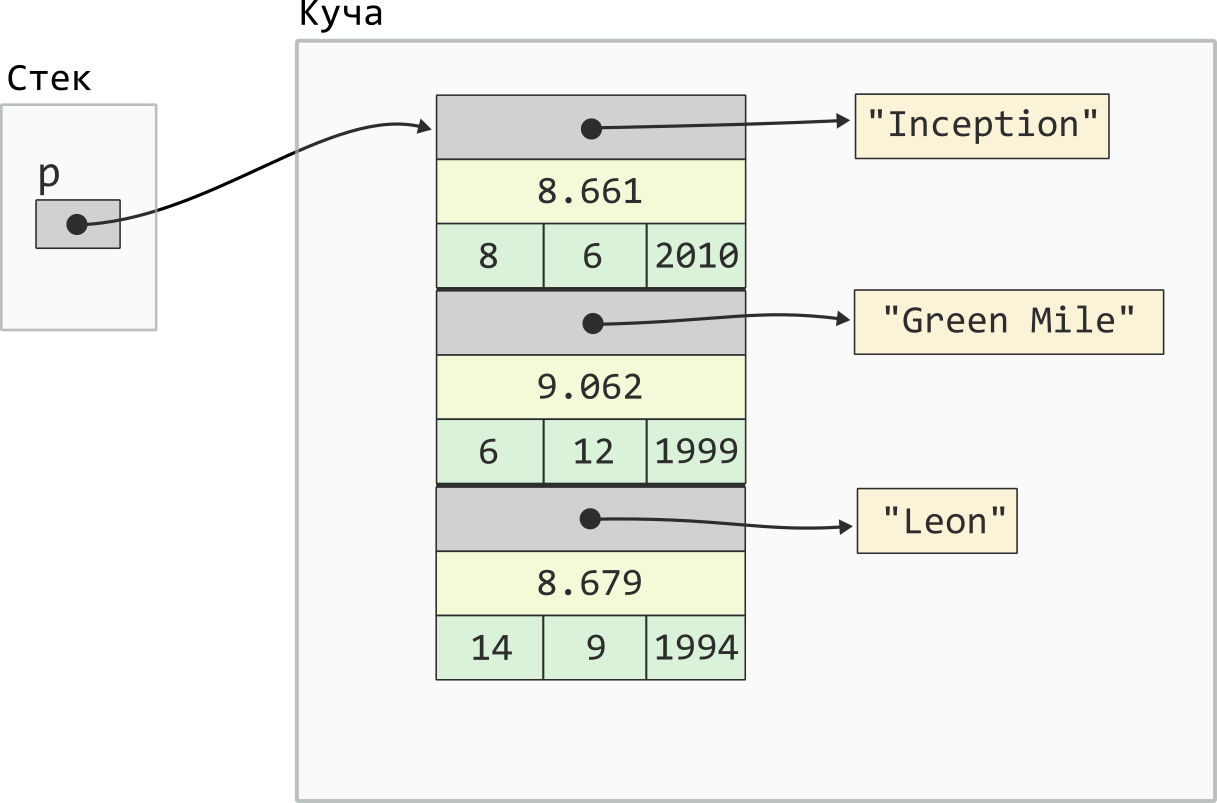
\includegraphics[scale=1]{../../images/pointer_schemes/pointer_to_array_of_struct_movie_charpointers.png}
\end{center}

\begin{center}
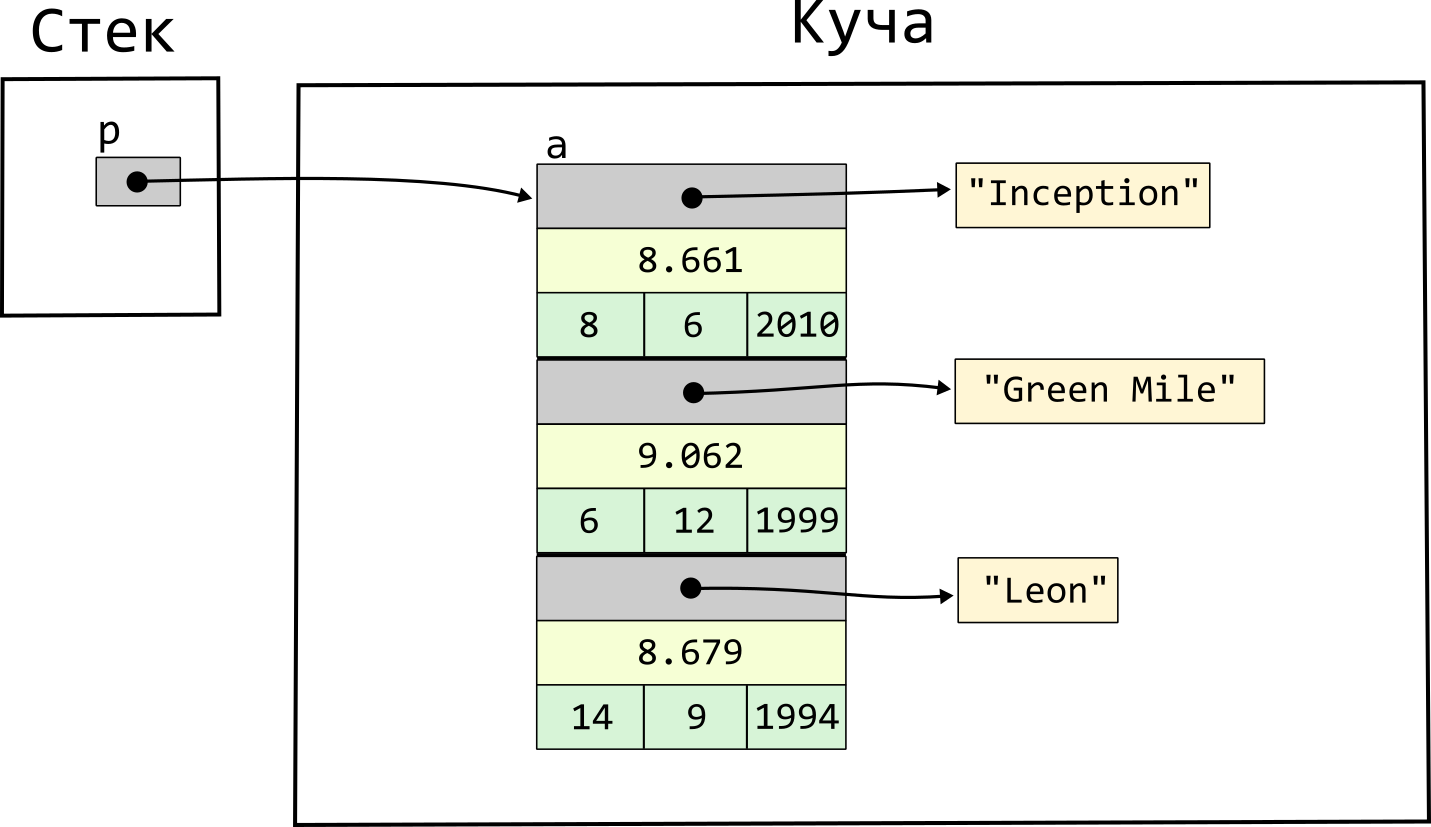
\includegraphics[scale=1]{../../images/pointer_schemes/pointer_to_array_of_struct_movie_charpointers_segments.png}
\end{center}

\newpage



\end{document}
